\documentclass[tikz,border=5pt]{standalone}
\usepackage{amsmath, amssymb}
\allowdisplaybreaks
\usepackage{braket}         % \ket{}, \bra{}
\usepackage[UTF8]{ctex}
\usepackage{newtxtext,newtxmath} % Times-like 正文 + 数学字体（PRA/PRL 风格）
\usepackage{graphicx} % 添加图片支持
\usepackage{tikz}     % 添加TikZ支持
\usetikzlibrary{
  arrows.meta,              % 现代箭头（Stealth 等）
  decorations.pathmorphing  % 备用：波浪线等（目前未用）
}
% =========================================================
% 全局数学公式样式
% 所有 $...$ 默认使用 displaystyle
% 让 \Omega, \Delta, V_{ij} 更饱满
% =========================================================
\everymath{\displaystyle}

\begin{document}
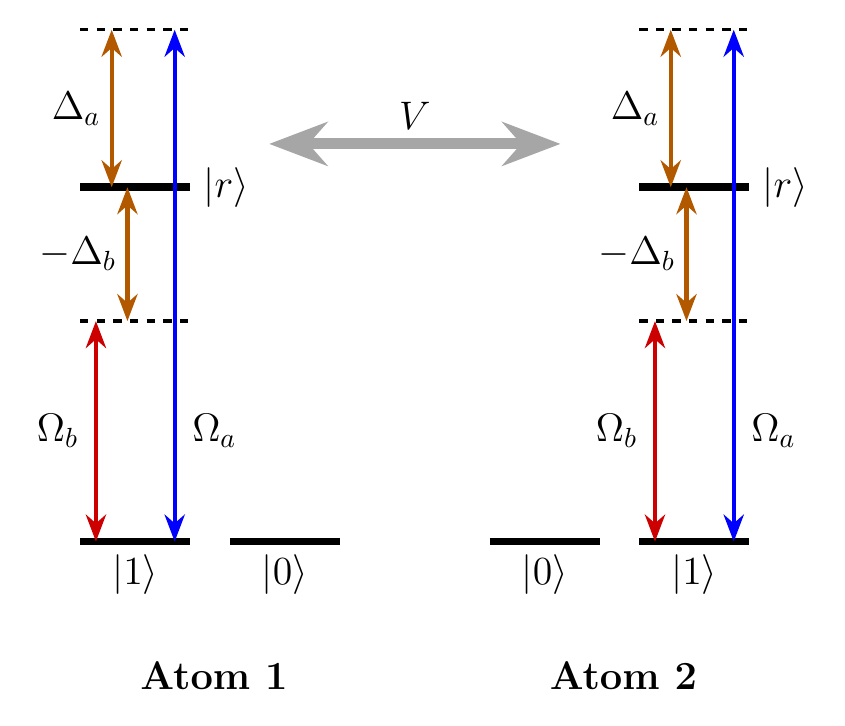
\begin{tikzpicture}[
    % =====================================================
    % 样式定义（只管"画笔属性"，不管几何）
    % =====================================================
    level/.style={
        line width=2.8pt          % 实能级：加粗实线
    },
    vlevel/.style={
        line width=1.2pt,
        dashed                   % 虚能级：细虚线
    },
    laser/.style={
        <->,
        line width=1.5pt,
        >=Stealth,               % 激光：双向箭头
        draw=blue
    },
    detune/.style={
        <->,
        line width=1.5pt,
        >=Stealth,               % 失谐 Δ：双向箭头
        draw=orange!70!black     % 使用更柔和的橙褐色
    },
    int/.style={
        <->,
        line width=4pt,
        draw=gray!70,
        >=Stealth                % Rydberg 相互作用
    },
    % =====================================================
    % 所有 node 的统一字体设置
    % =====================================================
    every node/.style={
        font=\Large\bfseries,
        text=black
    }
]

% =========================================================
% 全局几何参数（控制整体布局）
% =========================================================

% -------- 三个原子的横向位置 --------
\def\xA{0}        % Atom 1
\def\xB{5.2}      % Atom 2
\def\xC{10.4}     % Atom 3

% -------- 能级高度 --------
\def\yzero{0}     % |0>, |1> 基态

\def\yr{4.5}      % |r> 实能级

% -------- 虚能级高度 --------

\def\yrv{6.5}     % |r> 对应虚能级
\def\yrvb{2.8}   % 红失谐对应下方虚能级

% -------- 能级线长度 --------
\def\Lreal{1.4}  % 实能级长度（更长）
\def\Lvirt{\Lreal}  % 虚能级长度与实能级一致
\def\yOmegaLabel{1.4} % Omega 标签统一高度（对齐到原来 Omega_b 高度）

% =========================================================
% ===================== Atom 1 =============================
% =========================================================

% -------- 基态 |0>, |1> --------
\draw[level] (\xA,\yzero) -- ++(\Lreal,0)
    node[midway,below] {$\ket{1}$};

\draw[level] (\xA+1.9,\yzero) -- ++(\Lreal,0)
    node[midway,below] {$\ket{0}$};

% -------- 激发态 |A>, |r> --------

\draw[level] (\xA,\yr) -- ++(\Lreal,0)
    node[right] {$\ket{r}$};

% -------- 虚能级（激光失谐后的能级） --------

\draw[vlevel] (\xA,\yrv) -- ++(\Lvirt,0);
\draw[vlevel] (\xA,\yrvb) -- ++(\Lvirt,0);

% -------- 激光驱动 --------


\draw[laser, blue]
    (\xA+1.2,\yzero) -- (\xA+1.2,\yrv)
    node[right] at (\xA+1.28,\yOmegaLabel) {$\Omega_a$};

\draw[laser, red!80!black]
    (\xA+0.2,\yzero) -- (\xA+0.2,\yrvb)
    node[left] at (\xA+0.12,\yOmegaLabel) {$\Omega_b$};

% -------- 失谐标注 Δ --------


\draw[detune]
    (\xA+0.4,\yr) -- (\xA+0.4,\yrv)
    node[midway,left] {$\Delta_a$};

\draw[detune]
    (\xA+0.6,\yrvb) -- (\xA+0.6,\yr)
    node[midway,left] {$-\Delta_b$};

% -------- 原子标签 --------
\node at (\xA+1.7,-1.7) {Atom 1};

% =========================================================
% ===================== Atom 2 =============================
% =========================================================
% （结构与 Atom 1 完全一致，仅横向平移）

\draw[level] (\xB,\yzero) -- ++(\Lreal,0)
    node[midway,below] {$\ket{0}$};

\draw[level] (\xB+1.9,\yzero) -- ++(\Lreal,0)
    node[midway,below] {$\ket{1}$};



\draw[level] (\xB+1.9,\yr) -- ++(\Lreal,0)
    node[right] {$\ket{r}$};


\draw[vlevel] (\xB+1.9,\yrv) -- ++(\Lvirt,0);
\draw[vlevel] (\xB+1.9,\yrvb) -- ++(\Lvirt,0);


\draw[laser, blue]
    (\xB+3.1,\yzero) -- (\xB+3.1,\yrv)
    node[right] at (\xB+3.18,\yOmegaLabel) {$\Omega_a$};

\draw[laser, red!80!black]
    (\xB+2.1,\yzero) -- (\xB+2.1,\yrvb)
    node[left] at (\xB+2.02,\yOmegaLabel) {$\Omega_b$};



\draw[detune]
    (\xB+2.3,\yr) -- (\xB+2.3,\yrv)
    node[midway,left] {$\Delta_a$};

\draw[detune]
    (\xB+2.5,\yrvb) -- (\xB+2.5,\yr)
    node[midway,left] {$-\Delta_b$};

\node at (\xB+1.7,-1.7) {Atom 2};


% =========================================================
% ================= Rydberg 相互作用 =======================
% =========================================================

% -------- 最近邻相互作用 --------
\draw[int]
    (\xA+2.4,\yrv-1.45) -- (\xB+0.9,\yrv-1.45)
    node[midway,above] {$V$};

\end{tikzpicture}

\end{document}